\documentclass{beamer}
\usetheme{metropolis}

\usepackage{standalone}
\usepackage{circuitikz}
\usepackage{rotating}
\usepackage{float}
\usepackage{cleveref}
\usepackage{biblatex}
\addbibresource{plasma-chamber-presentation.bib}

\title{Ignition and Extinction Voltages of a Low Pressure Capacitively Coupled Plasma of Air}
\date{\today}
\author{David Nacouzi and Daniel Underwood}
\institute{North Carolina State University}
\begin{document}
  \maketitle
  
  % Section on background information
  \section{Quick Introduction to Plasmas}
  
  \begin{frame}{What is a Plasma?}

	``A plasma is a quasineutral gas of charged and neutral particles which exhibits
	collective behavior'' \footfullcite{Chen1984}
    
    \begin{itemize}
    	\item Frequently referred to as fourth state of matter
        \item Consists of (singly or more) ionized nuclei and electrons
    \end{itemize}
    
    \begin{figure}
        \begin{center}
        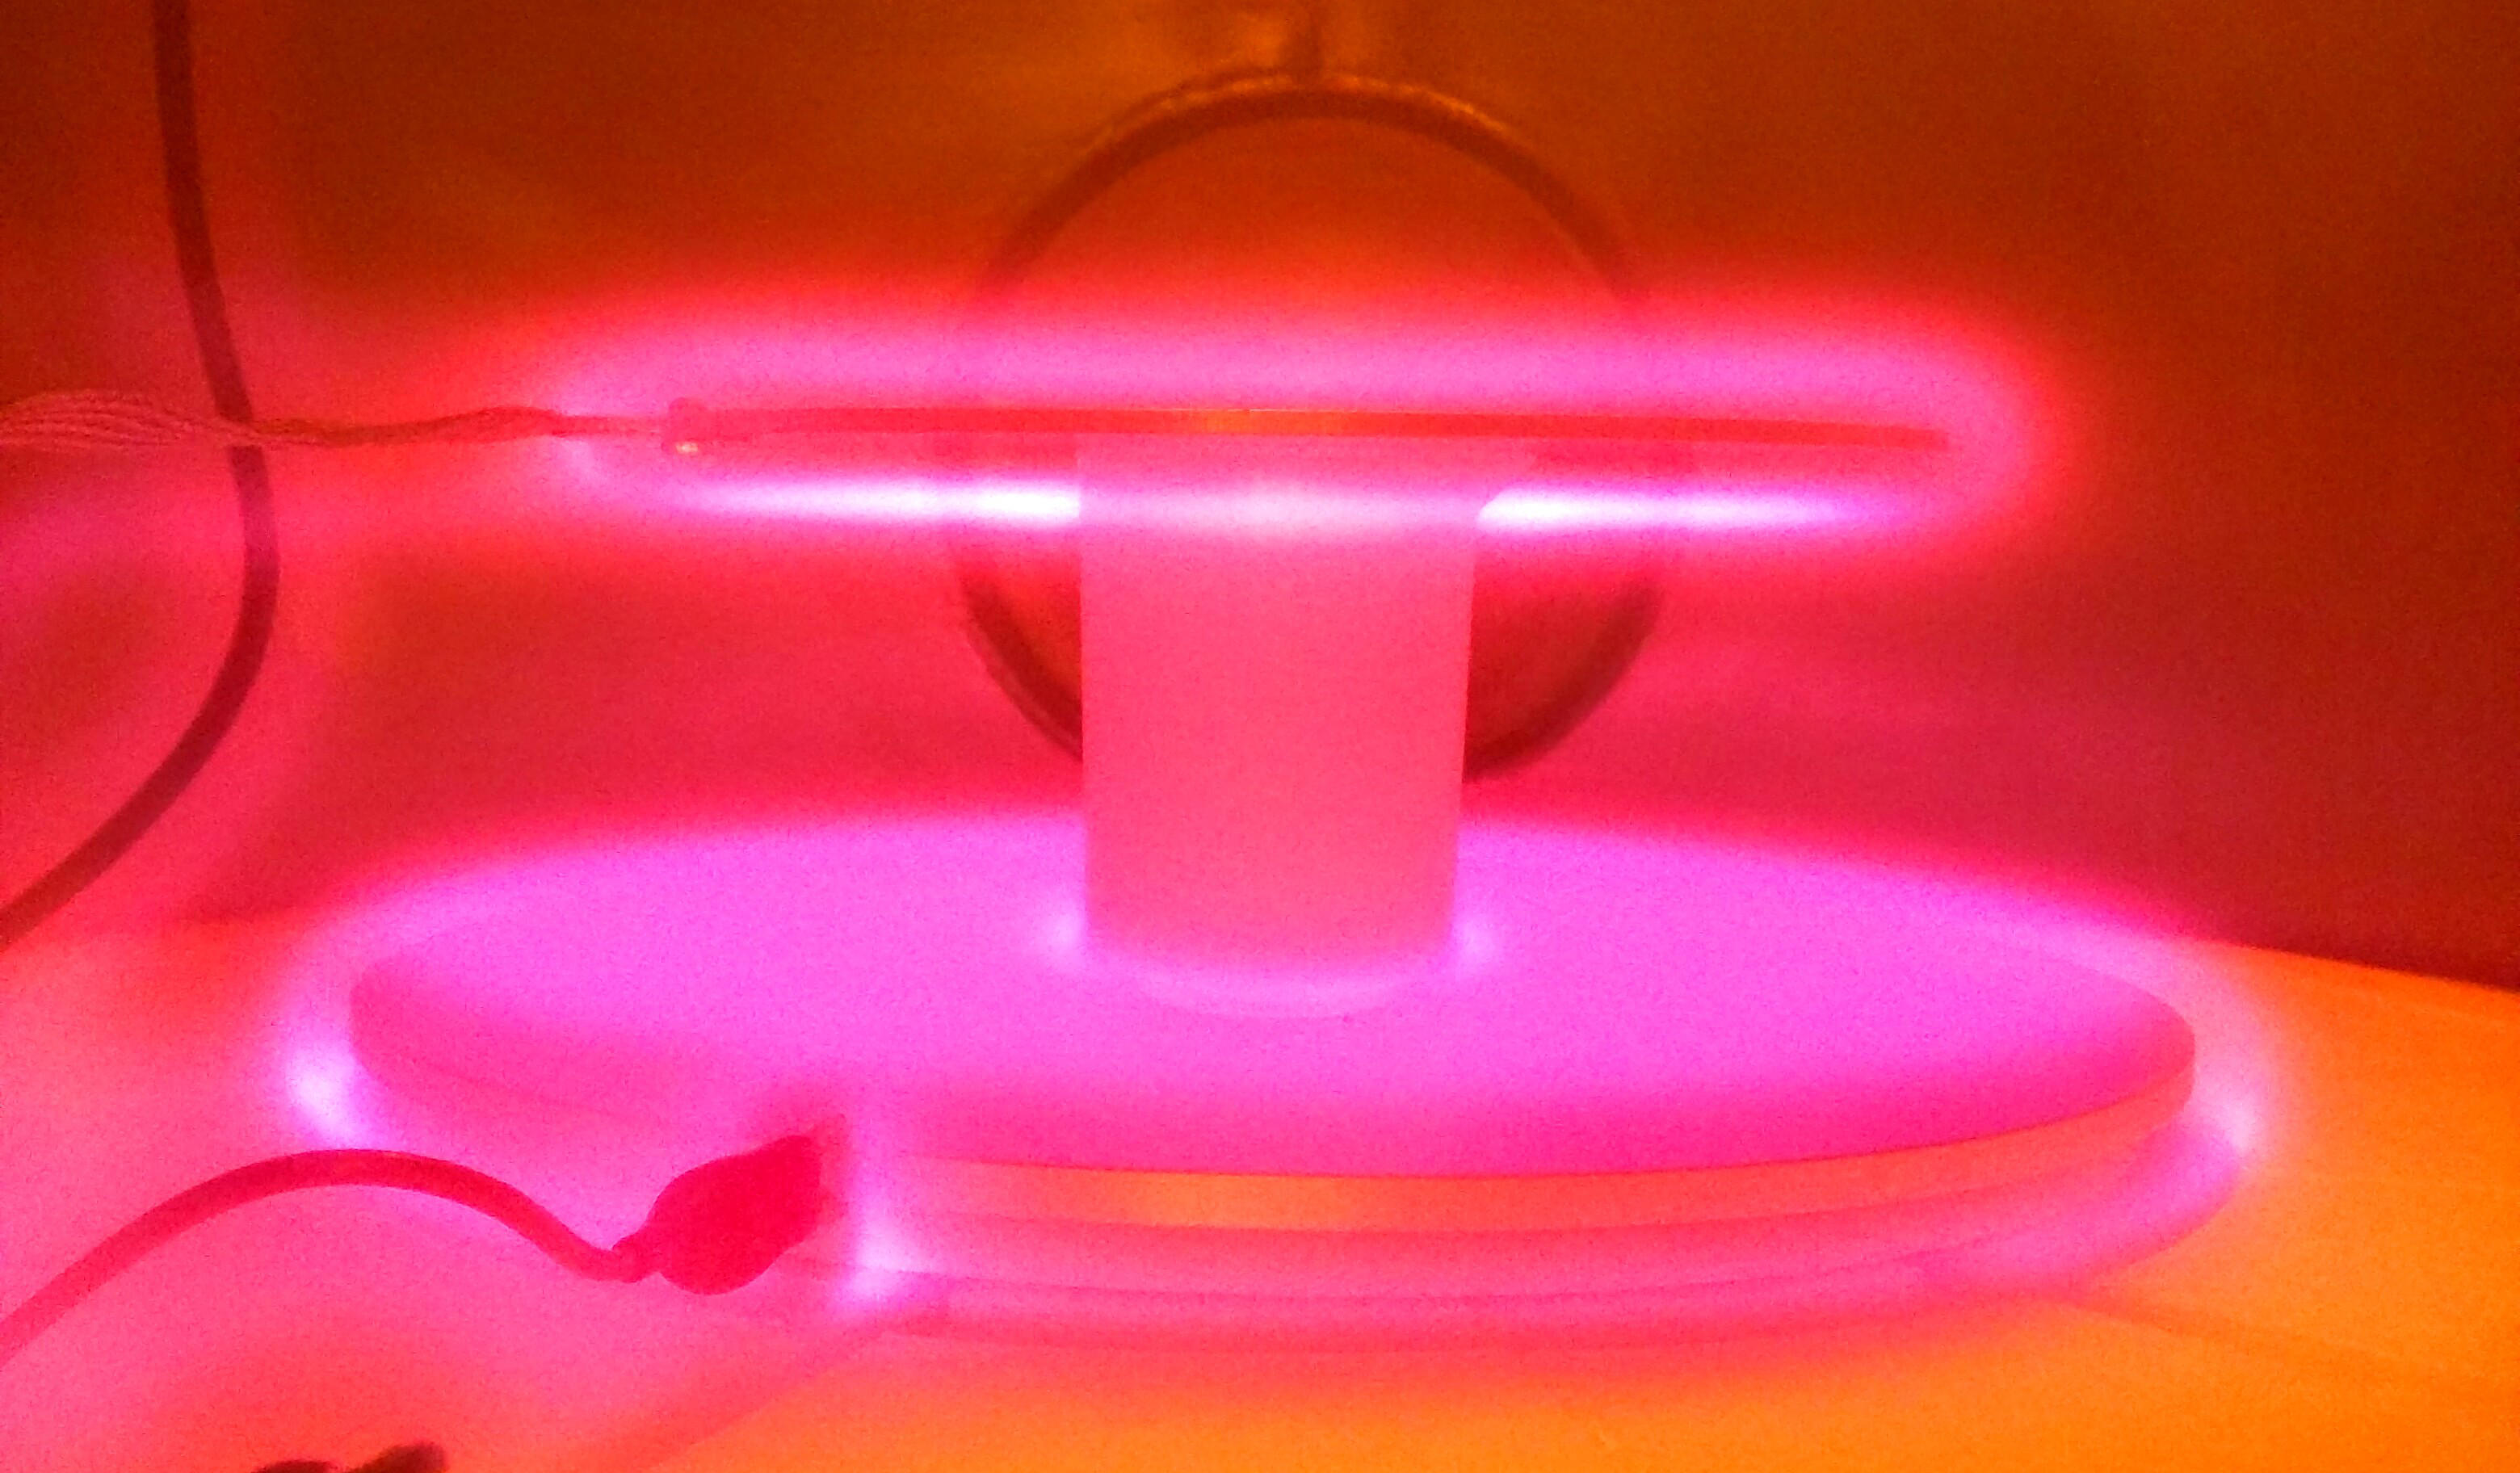
\includegraphics[width=0.25\textwidth, angle=-90]{../resources/plasma-sheath.png}
        \hspace{15pt}
        \caption{Glow Discharge}
        \label{fig: plasma-chamber}
        \end{center}
     \end{figure}
    
    
  \end{frame}
  
  \begin{frame}{Why Study Plasmas?}
  
    Plasmas are the most abundant type of normal matter in the universe and are present
    in stars, galaxies, and interstellar media
    
    \begin{itemize}
      \item Theory -- Meeting of fluid dynamics and electrodynamics
      \item Industry -- Numerous uses including materials processing
      \item Exploration -- Space travel and satellites
    \end{itemize}

  \end{frame}
  
  % Section on our setup and experiment
  \section{Our Experiment}
  
  \begin{frame}{Experimental Setup}
 
        % Description of plasma chamber and equipment
        \begin{figure}[H]
        \begin{center}
        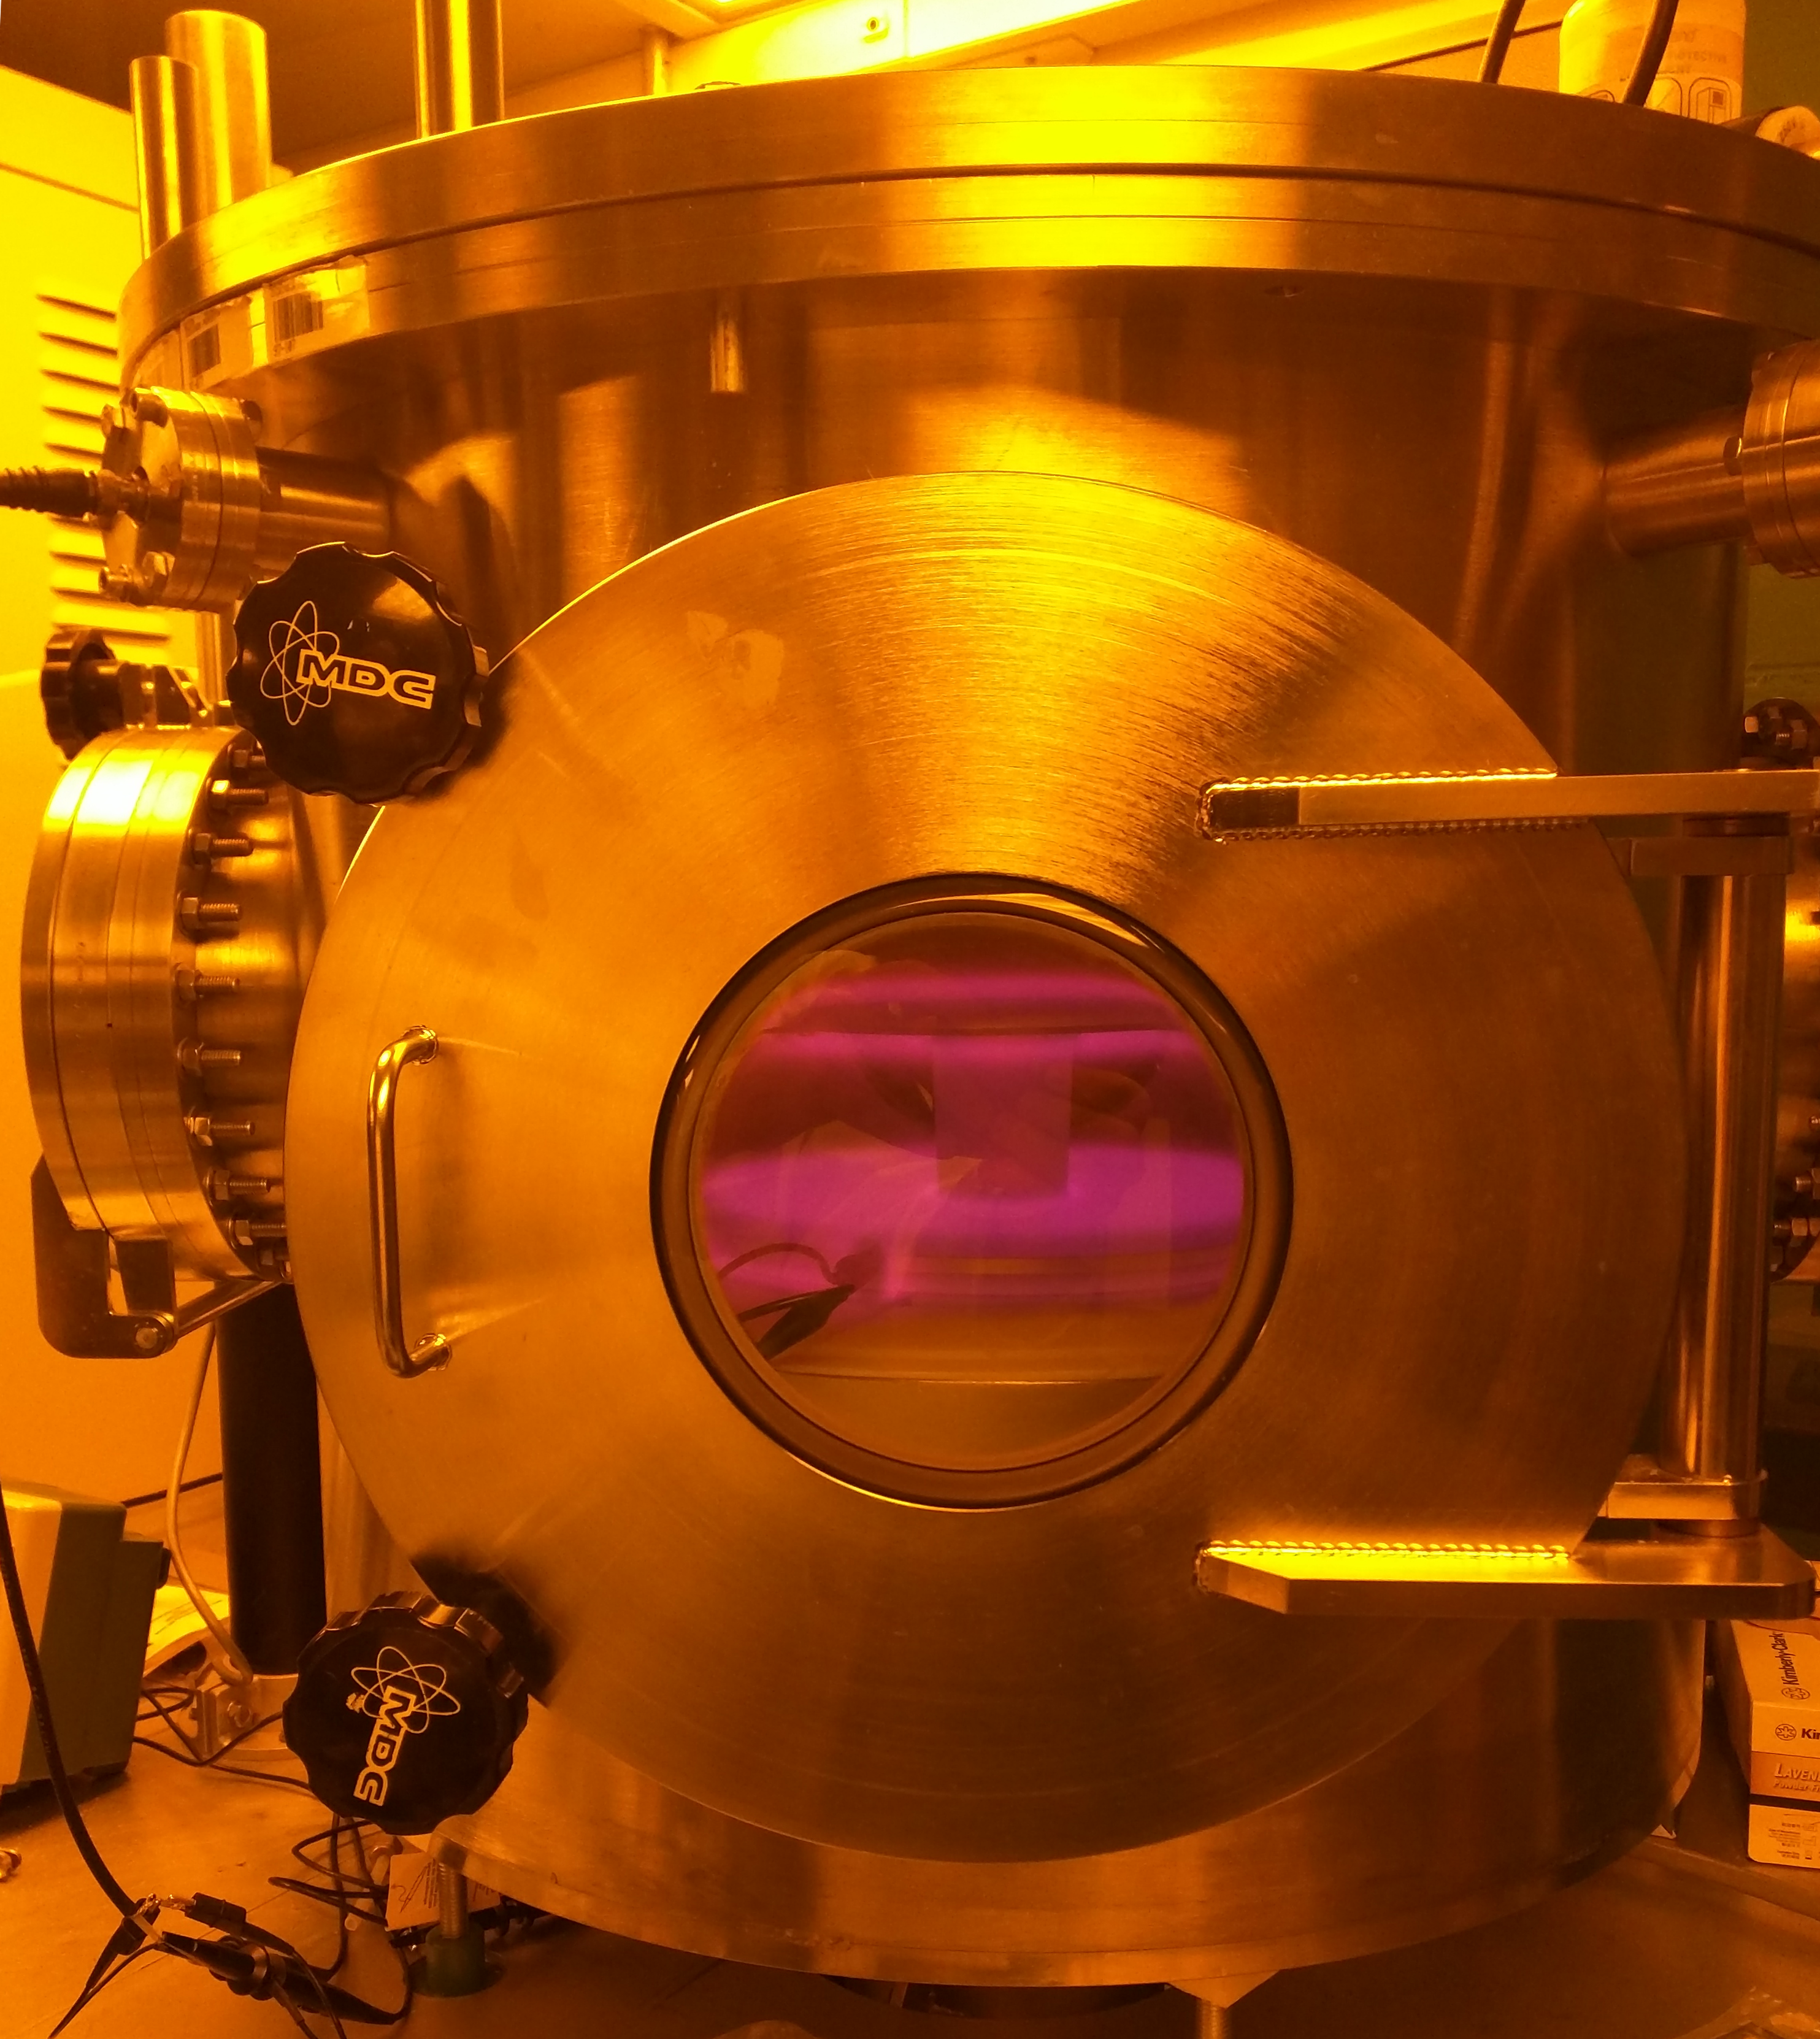
\includegraphics[width=0.3\textwidth]{../resources/plasma-chamber.png}
        \hspace{15pt}
        \includestandalone{../resources/plasma-chamber-diagram}
        \caption{Plasma Chamber Image and Diagram}
        \label{fig: plasma-chamber}
        \end{center}
        \end{figure}

     	\begin{itemize}
        	\item Vacuum chamber at vacuum on order of $10^{-1}\:\rm{Torr}$
            \item Two ``capacitor'' plates connected to $13.56\:\rm{MHz}$ power supply
            \item Probe to measure voltage between two plates
            \item Manually recorded statistical uncertainties by max deviation from mean within interval
        \end{itemize}

  	\end{frame}
  
  \begin{frame}{Expected Results}
  \begin{columns}
  	\begin{column}{0.4\textwidth}
  	\begin{center}
      \begin{figure}[H]
      \includegraphics[width=\textwidth]{../resources/paschen-curves.png}
      \caption{Paschen's Curves for Various Gases\footnotemark}
      \label{fig: paschens-curves}
      \end{figure}
    \end{center}
    \end{column}
    
    \footnotetext{\fullcite{paschen-curves}}
    
    \begin{column}{0.6\columnwidth}
    Expect breakdown (ignition) voltage to follow Paschen's Law:
    
    
    \begin{equation}
    V_B = \frac{B p d}{\ln{\left( A p d \right)} - \ln{\left[ \ln{\left( 1 + \gamma_{\rm{se}}^{-1} \right)} \right]}}
    \label{eqn: paschen-law}
    \end{equation}
    \end{column}
  \end{columns}
  
  \end{frame}
  
  \begin{frame}{Results}
  	% Discussion of results
    \begin{figure}
    \includegraphics[width=0.9\textwidth]{../resources/ignition-extinction.pdf}
    \caption{Obtained Ignition and Extinction Voltages}
    \end{figure}
  \end{frame}
  
  \begin{frame}{Results}
  	% Discussion of results
    \begin{figure}
    \includegraphics[width=0.9\textwidth]{../resources/paschen-fit.pdf}
    \caption{Obtained Fit}
    \end{figure}
  \end{frame}
  
  \begin{frame}{Results}
  
    Results suggestive of success in testing Paschen's Law, but not conclusive.
    
    \begin{itemize}
    \item Line of fit similar to known Paschen Curves.
    \item Attempted fit: $f(x) = \frac{Bx}{\log{\left( Ax \right)} - C}$
    
   \begin{center}
    \begin{tabular}{||c c c c||} 
      \hline
      Coefficient & Experimental Value & Fit Value & Uncertainty \\ [0.5ex] 
      \hline\hline
      A & 0.221& 0.311 & $\pm 5.61\times 10^{6}$ \\ 
      \hline
      B & 48.7& 32.9 & $\pm 23.5$ \\
      \hline
      C & 0.223& 0.301 & $\pm 1.80\times 10^{7}$ \\
      \hline
    \end{tabular}
    \end{center}
    
    \item Goodness-of-fit measurement:  ($\frac{\chi^2}{\nu}$) $\approx 0.37$
   
    
    \end{itemize}

  \end{frame}
  
  \begin{frame}{Discussion}
  
    Results suggestive of success in testing Paschen's Law, but not conclusive.
    
    \begin{itemize}
    \item $\alpha = \frac{1}{\lambda}$ applicable approximation
    \item Conducted most testing in "risky" region ($< 1\:\rm{Torr}$)
    \item Inhomogeneous electric field (plate size, inconsistent dielectric).
    
    \end{itemize}
   
   \end{frame}
   
  
  \begin{frame}{Future Improvements}
  \begin{itemize}
  \item Use same size electrode
  \item Use one sort of dielectric (hang top electrode)
  \item Increase pressure range
  \item Improve statistical uncertainties by automated data acquisition
  \item Explore inductively coupled plasmas
  
  \end{itemize}
  % Future improvements if time permits
  % Inductively coupled plasma, automated data collection
  \end{frame}
\end{document}
